\def\year{2017}\relax
%File: formatting-instruction.tex
\documentclass[letterpaper]{article}
\usepackage{aaai17}
\usepackage{times}
\usepackage{helvet}
\usepackage{courier}
\usepackage{graphicx}
\usepackage{multicol}
\usepackage{amsmath}
\frenchspacing
\setlength{\pdfpagewidth}{8.5in}
\setlength{\pdfpageheight}{11in}
\pdfinfo{
/Title (Insert Your Title Here)
/Author (Put All Your Authors Here, Separated by Commas)}
\setcounter{secnumdepth}{0}  
 \begin{document}
% The file aaai.sty is the style file for AAAI Press 
% proceedings, working notes, and technical reports.
%
\title{Data Synthesize for CNN on Skin Cancer Detection and Tracking}
\author{AAAI Press\\
Association for the Advancement of Artificial Intelligence\\
2275 East Bayshore Road, Suite 160\\
Palo Alto, California 94303\\
}
\maketitle
\begin{abstract}
 
\end{abstract}


\section{Introduction}


\section{Related Work}

% General
\cite{tensorflow}
\cite{ImageNet}

% Image Synthesis
\cite{PoissonImageEditing}
\cite{Render4CNN}
\cite{FlowNet}

% Detection
\cite{RCNN}
\cite{FastRCNN}
\cite{FasterRCNN}
\cite{R-FCN}

% Correspondence
\cite{SIFTFLow}
\cite{DeformableSpatialPyramid}
\cite{DenseCorrespondence3D}
\cite{StereoMatching}

\cite{FaceDetection-ConvNet-3D}
\cite{AtrousConv}
\cite{WarpNet}

\cite{VGGNet}

\cite{DoConvnetsLearnCorrespondence}
\cite{FullyConvolutionalNeuralNetwork}



\section{Data Synthesize}

\begin{figure*}[h!]
  \centering
  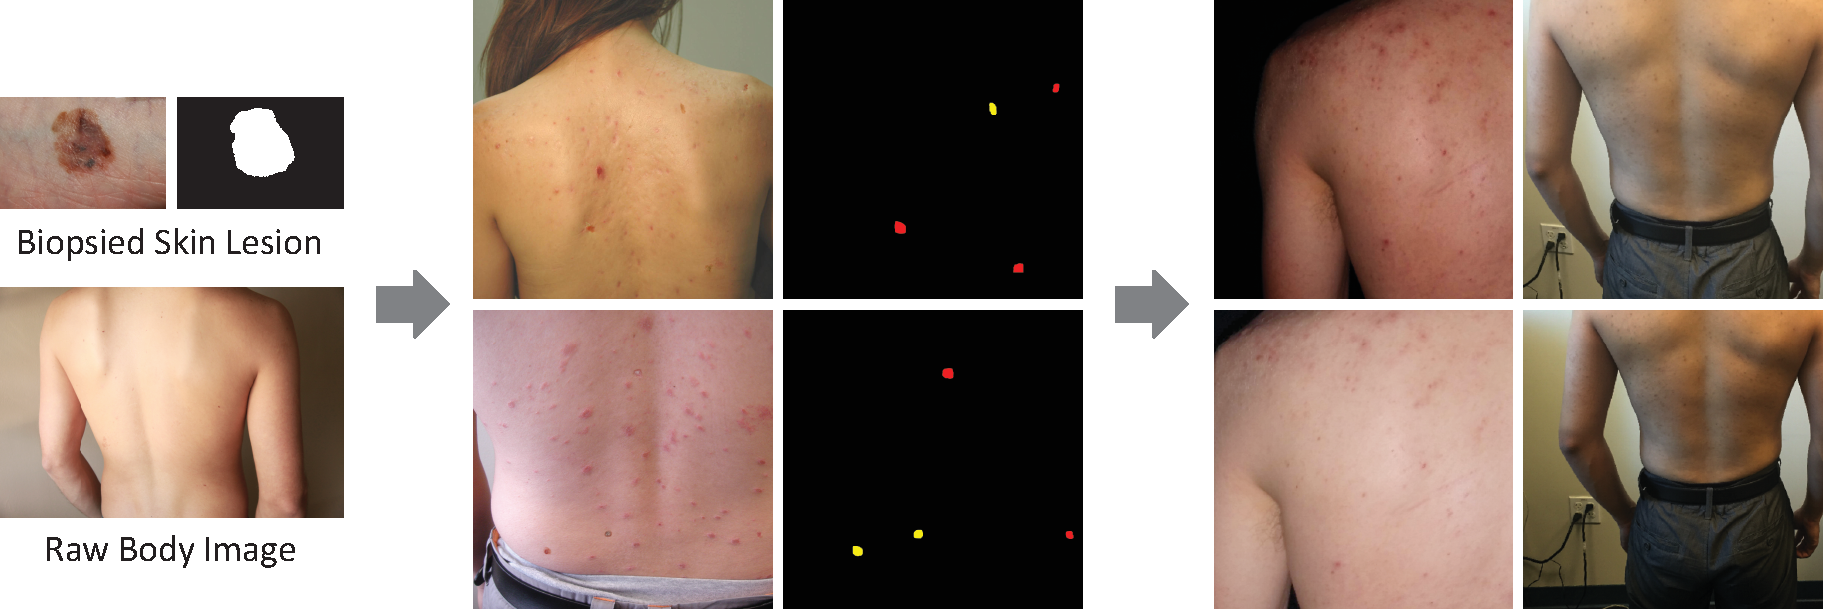
\includegraphics[width=\textwidth]{./blend.pdf}
  \caption{{\bf Samples of the generation pipeline.} (Left) Biopsied skin lesion with its mask and raw body image. (Middle) Generated training images for detection and corresponding label masks. The red areas in the label mask represent the blended malignant lesions, while the yellow areas represent the blended benign lesions. During training, the lesions are further subdivided into epidermal or melanocytic. (Right) Generated training images for tracking.}
  \label{fig:poisson}
\end{figure*}

A large dataset is an essential requirement for us to take advantage of data-driven methods like deep learning, which has been proven to perform extremely well in the field of computer vision (ref). For specific problems where high quality labeled images are hard to find, a scalable data synthesize method will be really helpful. We describe how we synthesize training images in the context of skin cancer detection and tracking in the following two sections.

\subsection{Image Generation for Detection}

To generate training data for detection, we augment real images with large area of skin with biopsied skin lesions using Poisson image editing. The biopsied skin lesions are obtained from Edinburgh Dermofit Image Library (ref). The main purpose is to simulate images taken at home or in clinical settings.

\subsubsection{Gradient Domain Image Blending}

Gradient Domain Fusion was first introduced in high dynamic range compression (Fattal et al. 2002) and image composition (Perez et al. 2003). The basic idea is to manipulate the gradient field instead of considering and changing the image intensity. This advantages of this idea is two-fold (Bhat et al. 2010): it is better for human perception, as the difference between intensities (i.e. gradient) is much more noticeable than intensity values; the other one is that we could have high-level control over images, since local change in gradient field could affect the global image.

Based on these considerations, we use Poisson image editing, which could seamlessly blend the skin images and the lesion by providing a mask to segment the lesion. If we use $\mathbf{v}$ as the gradient field of the source image (lesion), $\Omega$ as the corresponding masked area in the target image (skin), $\partial\Omega$ as the boundary of the masked area, $f^*$ as the known function of the target image, $f$ as the unknown function in area $\Omega$ that needs to be calculated. Then the problem can be formulated as optimizing:
\begin{align}
  \min_f \iint_\Omega |\nabla f - \mathbf{v}|^2 \text{ with } f|_{\partial\Omega} = f^*|_{\partial\Omega}
  \label{eqn:poisson}
\end{align}
where $\nabla\cdot = [\frac{\partial\cdot}{\partial x},\frac{\partial\cdot}{\partial y}]$ is the gradient operator, whose solution is the solution of a Poisson equation.

Edinburgh Dermofit Image Library has provided segmentation masks for each of their lesion images, thus is very convenient to use Poisson image editing. If the masks are not available, simple methods like adaptive threshold for segmenting the mask has proven to be working in our settings. 

\subsubsection{Feature Match for Choosing Blending Positions}

Poisson image editing will change the overall intensity of the skin lesion. In order not to change the intensity too much, we use the color histogram as feature to find match. 

We use RGB color space, dividing each of the axises into 8 bins. Thus we can calculate a cubic feature at a size of $8\times8\times8$ for every color image patches. We denote the value of the feature as $\{w_i\mid i = x\times64 + y\times8 + z, 1 \le x, y, z \le 8\}$, the total length of the feature as $L=512$.Then we normalize the feature and use the earth mover's distance (EMD) as the metric for comparing two features. We define $\mathbf{D} = [d_{i,j}]$, $d_{i,j} = |x_i - x_j| + |y_i - y_j| + |z_i - z_j|$, where $x_\cdot$ and $y_\cdot$ are the corresponding coordinate in the RGB axises. We denote the two features as ${w_i}$ and ${w_j}$, then the goal is to find flow $\mathbf{F} = [f_{i,j}]$, to minimize to overall cost:
\begin{align}
  EMD(P, Q) = \frac{\sum^L_{i=1}\sum^L_{j=1}f_{i,j}d_{i,j}}{\sum^L_{i=1}\sum^L_{j=1}f_{i,j}}
\end{align}
while subjected to the constraints that \par
$f_{i,j}\ge0, 1\le i\le L, 1\le j\le L$ \par
$\sum_{j=1}^L f_{i,j}\le w_i, 1\le i\le L$ \par
$\sum_{i=1}^L f_{i,j}\le w_j, 1\le j\le L$ \par
$\sum_{i=1}^L\sum_{j=1}^L f_{i,j} = \min(\sum_{i=1}^L w_i, \sum_{j=1}^L w_j)$

We resize the skin lesion image patch into appropriate size, then randomly select a position in a skin image. The color histogram features of surrounding area of the skin lesion (the black area in the top left corner of Figure~\ref{fig:poisson}) and the area of the same size as the skin lesion patch on the skin image are used for comparison. If the EMD is lower than a predefined threshold, we blend the lesion there.

Note that our choice is largely due to the model's simplicity and efficiency. More advanced blending algorithm like (a more advanced blending method) can be used, and one can also train a skin classifier to choose the blending positions. Some blending results along with the label mask of the attached lesions can be seen in Figure~\ref{fig:poisson}.

\subsection{Image Generation for Tracking}

To generate training data for tracking, we further augment the images generated in the last section by using several image distortion techniques. The main purpose is not to simulate the reality, but to force our network learn the correspondence between on by viewing the distorted local texture information.

\subsubsection{Lesion Distortion}

Skin lesions will change as the time pass by. We will simulate this by distorting the attached lesions from previous section. We randomly adjust the shape, size, brightness, along with removing them and attaching new lesions at a small probability. The coefficients of these transformation are all randomly set to increase diversity.

\subsubsection{Image Distortion}

Aside with lesion distortion, we also have to distort the image, as images can not be the same although the pose and view point are approximately the same. 

We use gamma correction with randomly set coefficient to distort the brightness. Then use elastic deformation as described in (ref). This is done by first generating random displacement fields, that is $\Delta x(x, y) = \text{rand}(-1, +1)$ and $\Delta y(x, y) = \text{rand}(-1, +1)$, where $\text{rand}(-1, +1)$ is a random number between $-1$ and $+1$, generated with a uniform distribution, then convolving with a Gaussian of a randomly decided standard deviation $\sigma$ (in pixels). Afterwards, we use perspective transformation with respect to randomly-sampled four points at the four corners of the images. We generate two distorted images using above techniques, then randomly crop from these two images at randomly sampled adjacent positions.

We could still have pixel-wise correspondence after all the distortion techniques described above. We use the correspondence as our label to train the network for tracking. Sample images could be seen in Figure~\ref{fig:poisson}.

\section{The Proposed System}

\begin{figure}
  \centering
  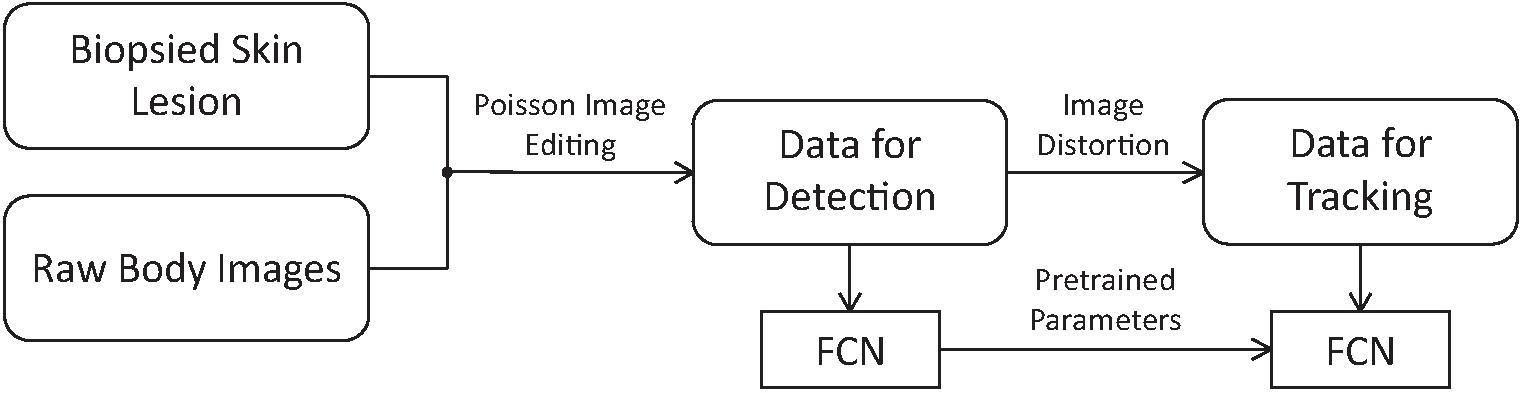
\includegraphics[width=0.5\textwidth]{./pipeline.pdf}
  \caption{\bf Overview of the proposed system.}
  \label{fig:pipeline}
\end{figure}

\begin{figure*}[h!]
  \centering
  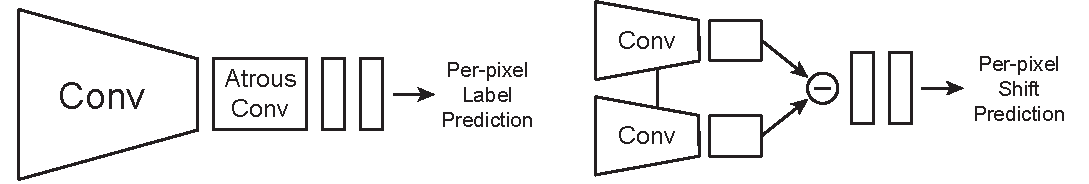
\includegraphics[width=\textwidth]{./network.pdf}
  \caption{\bf The structure of the neural network.}
  \label{fig:network}
\end{figure*}

\subsection{Skin Cancer Detection}

The skin lesions are not like the faces or pedestrians that can be separated into independent objects unambiguously. Many lesions like the inflammatory will link together to form an area, which will make it hard to identify each one of the lesions. Thus the main purpose of solving the task of skin cancer detection is to highlight the areas where are most suspicious of being a malignant cancer, that is, to tell the doctors or the consumers where to look at.

We would first do five-way classification at a pixel level using a customized fully convolutional neural network, then post processing the inference confidence map to high the suspicious lesions.

\subsubsection{Training Data Preparation}

The attached lesions are consisted of four types: epidermal malignant, epidermal benign, melanocytic malignant, melanocytic benign. For simplicity, we denote the four classes as "foreground". Besides the four classes, we use a fifth class "background" for other areas like skin, walls, pants, etc. We directly label every pixels in the attached area of the lesions as its corresponding class. However, for pixel level prediction, since the original raw body images may already contain lesions on them, we shall not label all the rest areas as "background", which will include tons of false labels.

To alleviate this problem as well as balancing between the "foreground" and "background", we first manually exclude areas where original lesions are very salient (this won't be a burden as hundreds of raw body images is enough to train a good detector), then randomly sample the same amount of pixels as the "foreground" over the rest area as the "background".

As we will use deep supervision for better discriminative feature training and better converge result, the label maps will be further downscaled to several different scales. We will use these label maps to supervise the learning process of our model. We denote $C = \{0, 1, 2, 3, 4\}$ as the class labels where $t = 0$ represents the background class. Assume there are $L$ levels of predictions, and at level $l$, we have $n_l$ chosen positions. We denote the position and label pairs in level $l$ as $\{(\mathbf{x}_i^l, t_i^l)^{n_l}_{i=1}\}$, where $\mathbf{x}_i^l = (x_i^l, y_i^l)$ is the 2D positions of the $i$th chosen point, and $t_i^l \in C$.

\subsubsection{Network Structure and Loss Function}

The structure of our network can be viewed in Figure~\ref{fig:network}. Fully convolutional neural network has been proven to be a very good model for pixel wise prediction. On top of it, many improvements have been proposed to further improve the performance, like (ref). 

In our model, we first downscale the feature maps while increasing the number of channels using stacked layers of typical convolution. Then we deconvolute the feature map while incorporating the concept of skip link (ref) to concatenate the deconvolution results with the features from the contractive part of the network.

In order to make the learned features from the middle layers of the model more discriminative, we add a convolutional layer to calculate the final prediction from the features of different scales at the deconvolutional part. Then we add the loss of each prediction level together with different weights. On each position $\mathbf{x}^l_i$, our model will calculate a discrete probability distribution $p^{\mathbf{x}^l_i} = (p_0^{\mathbf{x}^l_i}, p_1^{\mathbf{x}^l_i}, \cdots, p_4^{\mathbf{x}^l_i})$, representing the probability over the $5$ classes. If we denote the weight at each level as $\{w_l\mid 1\le l \le L\}$, we have the loss
\begin{align}
  \mathcal{L}_{detection} = -\sum_{l=1}^L \frac{w_l}{n_l} \sum_{i=1}^{n_l} \log{(p_{t_i^l}^{\mathbf{x}^l_i})}
\end{align}
The weights $\{w_l\}$ are set manually, and the value is usually becoming larger as $l$ goes higher. Intuitively, the coarser the prediction, the more accurate the neural network should be, and this is also a way to force the network to be more discriminative at a earlier stage.

\subsubsection{Saliency Aware Post Processing}

Some samples of the raw prediction results are shown as (b) in Figure~\ref{fig:raw_results}. Based on the principle that to make the suspicious places salient to the doctors, we use the following post processing techniques to make the confidence map look more organized and meaningful:
\begin{enumerate}
  \item[1)] We first calculate the connected components with respected to 4-adjacent connection.
  \item[2)] Then eliminate those components who hold a size less than a predefined threshold.
  \item[3)] Then change each connected component into its own convex hull.
  \item[4)] Then use the ratio between malignant pixels and all foreground pixels inside the convex hull as the probability of being a malignant lesion.
\end{enumerate}

The results can be seen at (c) in Figure~\ref{fig:raw_results}. We then use this inference results to calculate the precision and recall curve on real clinical images. 

\begin{figure*}[h!]
  \centering
  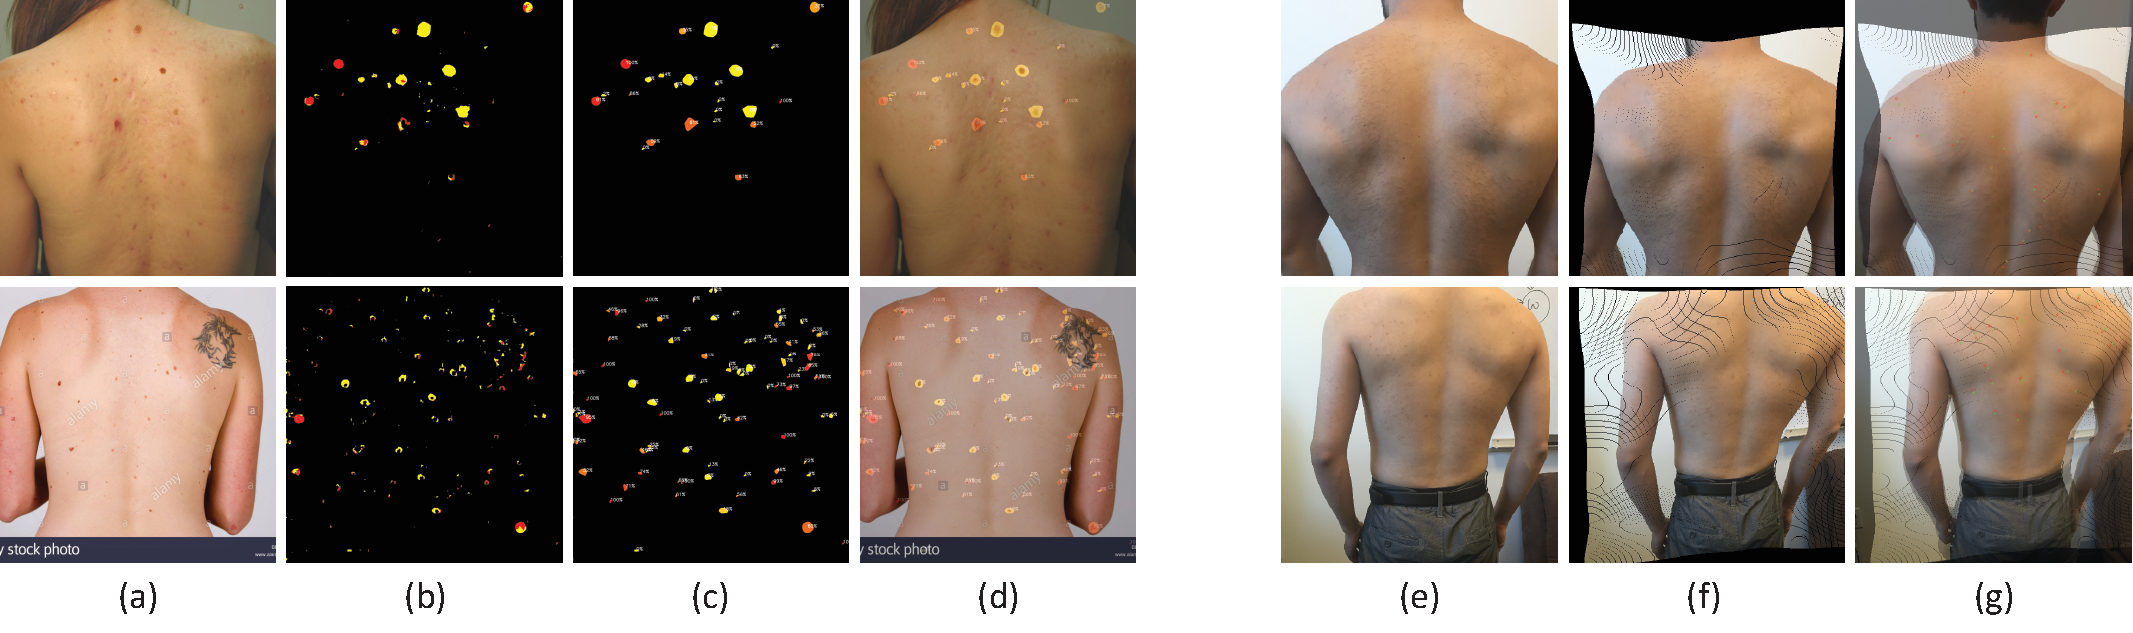
\includegraphics[width=\textwidth]{./raw_results.pdf}
  \caption{{\bf Samples of the results generated from each stage of our system.}}
  \label{fig:raw_results}
\end{figure*}

\subsection{Skin Cancer Tracking}

(Some words to describe the tracking procedure in a high-level way.)

\subsubsection{Training Data Preparation}

As described in the section of Data Synthesize, all the distorted image pairs have pixel-wise correspondence. Since we will use approximately the same model as detection, the correspondence label maps is further downscaled to $L$ different scale for supervising the training of our model. Unlike the label map for detection, all the positions will be chosen for back propagate the loss. We denote $(\mathbf{x}^l_i, \mathbf{t}^l_i)$ as the data of position $i$ on $l$th level, where $\mathbf{x}^l_i = (x^l_i, y^l_i)$ is the 2D position of this point, and $\mathbf{t}^l_i = (\Delta x^l_i, \Delta y^l_i)$ is the label to this position.

\subsubsection{Network Structure and Loss Function}

The network is identical to the network for detection, except that we combine the two images together to form a tensor of channel $6$ instead of channel $3$ as input.

On each position $\mathbf{x}^l_i$, our model will calculate a shift $\mathbf{d}^l_i = (dx^l_i, dy^l_i)$, we have the loss
\begin{align}
  \mathcal{L}_{tracking} = \sum_{l=1}^L \frac{w_l}{n_l} \sum_{i=1}^{n_l}
  \lVert \mathbf{t}^l_i - \mathbf{d}^l_i \rVert
\end{align}
where $\{w_l\mid 1\le l \le L\}$ is the weights to each level, and $\lVert \cdot \rVert$ represents the $l_2$-norm, which is the same as calculating the Euclidean distance between the labels and the predictions.


\section{Experiments}

\subsection{Detection}

The materials we use for synthesizing the detection training set is 500 high-res skin images scrapped from Internet and 1,300 high quality skin lesion images from Edinburgh Dermofit Library (ref). The lesions span across ten different classes including melanomas, seborrhoeic keratosis and basal cell carcinomas, and each of them has a gold standard diagnosis based on expert opinion (including dermatologists and dermatopathologists).


\subsection{Tracking}


\section{Conclustion}


\bibliographystyle{aaai}
\bibliography{ref}
\end{document}
